\chapter{Linear and K-NN Models}

\section{Linear models}

\subsection{Univariate Linear Regression}

\subsubsection{Unidimensional Input}
The simplest form of regression, with one input variable $x$, and one output variable $y$. We assume a model expressed as:

\begin{equation*}
    h_w(x) = w_1 x + w_0
\end{equation*}

where $w_0$ and $w_1$ are real-valued coefficients (or parameters/weights). This hypothesis corresponds to a simple line. Learning such a function with LMS (least mean squares) means finding the $w$ that minimize the residual sum of squares; i.e., find $argmin_w E(w)$ in $L_2$ (where $E(w) = \frac{1}{l}\sum_{p=1}^l (y_p - h_w(x_p))^2$).

In order to find such value of $w$, we must find the local minimum of the error function, corresponding to the point where the gradient is equal to 0:

\begin{equation*}
    \dfrac{\partial E(w)}{\partial w_i} = 0, i = 1, ..., n+1
\end{equation*}
For the univariate case, $w$ has dimension = 2, so we must search the value of $w$ such that:

\begin{center}
    $\dfrac{\partial E(w)}{\partial w_0} = 0$, $\dfrac{\partial E(w)}{\partial w_1} = 0$.
\end{center}
Below is how the partial derivative of $E(w)$ is calculated for a generic $w_i$:

\begin{equation*}
\dfrac{\partial E(w)}{\partial w_i} = 2 \sum_{p=1}^l (y_p - h_w(x_p)) \cdot \dfrac{\partial (y_p - h_w(x_p)}{\partial w_i} = \boxed{2 \sum_{p=1}^l (y_p - h_w(x_p)) \dfrac{\partial (y_p - w_0 - w_1x)}{\partial w_i}}
\end{equation*}

By calculating for $w_0$ and $w_1$, we get:

\begin{equation*}
\dfrac{\partial E(w)}{\partial w_0} = -2 \sum_{p=1}^l (y_p - h_w(x_p))
\end{equation*}
\begin{equation*}
\dfrac{\partial E(w)}{\partial w_1} = -2 \sum_{p=1}^l (y_p - h_w(x_p)) \cdot x.
\end{equation*}

\subsubsection{Multidimensional Input}
When the input has dimension $n>1$, the function $h_w(x)$ can be expressed as:
\begin{equation*}
    h_w(x) = w_0 + \sum_{i=1}^n w_i x = w_0 + w_1x_1 + w_2x_2 + ... + w_nx_n = \boxed{w^T x + w_0}
\end{equation*}

$w_0$ is often called the \textbf{intercept/threshold/bias/offset...}, since $h_w(x) = 0$ is equivalent to $w^T x = -w_0$.

\subsection{Classification}
The same model(s) used for regression can be used for classification as well. Given a set of $l$ points, equally distributed in two classes, we want to find an \textbf{hyperplane}, represented by $w^Tx + w_0$, that can help decide whether a new point belongs to one class or the other. The function to approximate will be in the form:

\begin{center}
    $h_w(x) = sign(w^Tx + w_0)$\hfill
    \text{or, alternatively,\hfill}
    $h_w(x) = \begin{cases}
                1 & \text{if } w^Tx \geq -w_0 \\
                0& \text{otherwise}
            \end{cases}$
\end{center}
both of whom classify a point depending on where it sits with respect to the defined decision boundary. 

\subsection{Learning Algortihms}

The following section will present two learning algorithms, both using a linear model and based on LMS.
The first algorithm uses a direct approach, based on the normal equation solution. The second algorithm offers an iterative solution based on gradient descent.

The first step is redefining the learning problem and the loss. Assuming a classification problem:

\begin{itemize}
    \item \textbf{Given}: a set of $l$ examples $(x_p, y_p)$, and a loss function $L$

    \item \textbf{Find}: The weight vector $w$ that minimizes the expected loss on the training data $R_{emp} = \dfrac{\sum_{p=1}^l L(h_w(x_p), y_p)}{l}$
\end{itemize}
Let's assume error is being calculated by using least squares (as for the regression), so $E(w) \propto \sum_{p=1}^l (y_p - w^Tx_p)^2$.

The issue with trying to minimize the expected loss is that using a piecewise constant function to calculate it's value can make it a difficult problem, since the function is not differentiable. The solution is to "soften" the loss function by using a smooth, differentiable function instead.

The problem can be reformulated as:

\begin{itemize}
    \item \textbf{Given}: as above

    \item \textbf{Find}: find $w$ to minimize the residual sum of squares:

    $E(w) = \sum_{p=1}^l (y_p - x_p^Tw)^2 = ||y-Xw||^2$,

    where X is a matrix $l \times n$ where each row is an input vector $x_p$.
\end{itemize}

Since this (differentiable) error function is quadratic, the minimum error always exists (but may not be unique). Let's differentiate the function:

\begin{equation*}
\begin{gathered}
    \dfrac{\partial E(w)}{\partial w_j} = \dfrac{\partial \sum_{p=1}^l (y_p - x_p^Tw)^2}{\partial w_j} = 2\sum_{p=1}^l (y_p - x_p^Tw) \cdot \dfrac{\partial (y_p - x_p^Tw)}{w_j} = \\ 2\sum_{p=1}^l (y_p - x_p^Tw) \cdot (\dfrac{\partial y_p}{\partial w_j} - \dfrac{\partial x_{p,1}w_1}{\partial w_j} - \dfrac{\partial x_{p,2}w_2}{\partial w_j} - \dots - \dfrac{\partial x_{p,n}w_n}{\partial w_j}) = \\ \boxed{-2\sum_{p=1}^l (y_p - x_p^Tw)^2 \cdot x_{p,j}}
\end{gathered}
\end{equation*}

The gradient can be also expressed as:
\begin{equation*}
    \dfrac{\partial E(w)}{\partial w_j} = -2\sum_{p=1}^l \delta_p \cdot s_{p,j}
\end{equation*}
This form will be used later.

\subsubsection{Singular Value Decomposition (direct approach)}
We can get the \textbf{normal equation} (the point with gradient of $E$ equal to 0):

\begin{equation*}
(X^TX)w = X^Ty
\end{equation*}
If $X^TX$ is not singular, then the unique solution is given by:

\begin{equation*}
    w = (X^TX)^{-1}X^Ty = X^+y
\end{equation*}
where $X^+$ is the \textbf{Moore-Penrose pseudoinverse} of X.

If $X^TX$ is singular, then the solutions are infinite. The \textbf{singular value decomposition (SVD)} can be used to compute this pseudoinverse:

\begin{equation*}
    X = U\Sigma V^T \implies X^+ = V \Sigma^+U^T
\end{equation*}

where $\Sigma$ is the diagonal, and $\Sigma^+$ is the diagonal where all nonzero entries are replaced by their reciprocal. Moreover, we can apply SVD directly to calculate $w = X^+y$.

\subsubsection{Gradient Descent (iterative approach)}

The \textbf{gradient} is the ascent direction; it expresses in which direction the error function grows. So, by moving with a \textbf{gradient descent}, we can gradually move towards the minimum of the function. The search begins with some initial values given to the weight vector, then the values are modified iteratively to minimize the error function (local search).

\begin{figure}[h]
    \centering
    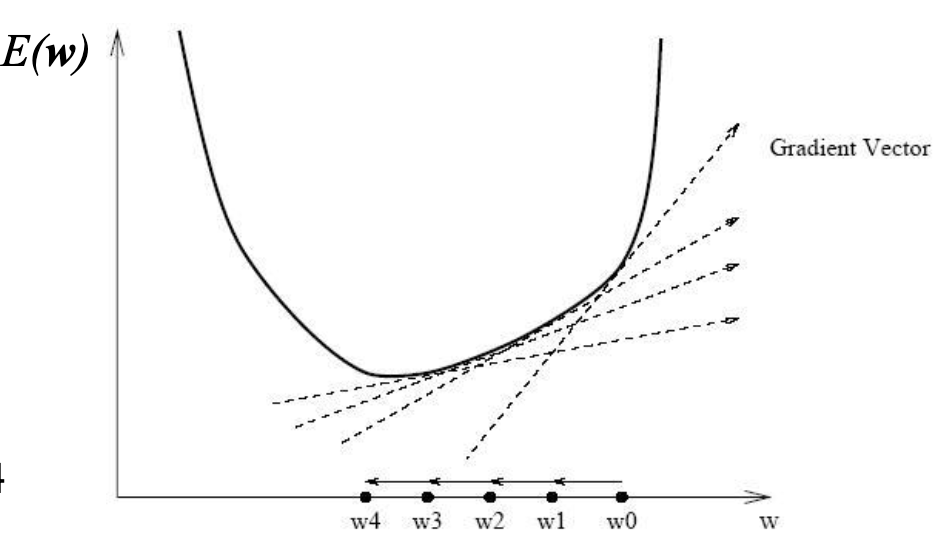
\includegraphics[width=0.5\linewidth]{img/gradient descent.png}
\end{figure}

So, for each iteration, the amount $w$ should be changed with is calculated as:

\begin{equation*}
    \Delta w = - \dfrac{\partial E(w)}{\partial w} =
    \begin{bmatrix}
    - \dfrac{\partial E(w)}{\partial w_1}\\
    - \dfrac{\partial E(w)}{\partial w_2}\\
    \dots\\
    - \dfrac{\partial E(w)}{\partial w_n}
    \end{bmatrix}
    =
    \begin{bmatrix}
    \Delta w_1\\
    \Delta w_2\\
    \dots\\
    \Delta w_n\\
    \end{bmatrix}
\end{equation*}

Each new value of $w$ will be calculated as: $w_{new} = w + \eta*\Delta w$, where $\eta$ is the \textbf{learning rate}: the "step size" that controls the speed of the gradient descent. The algorithm is the following:

\begin{enumerate}
    \item Start with $w_{initial}$ (small), fix value of $\eta \in [0,1]$

    \item Compute $\Delta w = \dfrac{\partial E(w)}{\partial w}$

    \item Compute $w_{new} = w + \eta*\Delta w$

    \item Repeat (2) and (3) until convergence, or $E(w)$ is sufficiently small.
\end{enumerate}
To use least mean squares, divide $\Delta w$ by $l$.

This way of calculating $w$ is called an \textbf{error correction rule} (also called \textbf{delta rule} since it refers to $\delta_p = y_p - x_p^Tw$), since it changes the value of $w$ proportionally to the error to "correct" it:

\begin{itemize}
    \item \bm{$(input_j > 0, error > 0)$} $\rightarrow$ $\Delta w$ is \textbf{+} $\rightarrow$ $w_j$ must be increased $\rightarrow$ increment output $\rightarrow$ \textbf{less error}

    \item \bm{$(input_j > 0, error < 0)$} $\rightarrow$ $\Delta w$ is \textbf{-} $\rightarrow$ $w_j$ must be decreased $\rightarrow$ reduce output $\rightarrow$ \textbf{less error}

    \item \bm{$(input_j < 0, error > 0)$} $\rightarrow$ $\Delta w$ is \textbf{-} $\rightarrow$ $w_j$ must be decreased $\rightarrow$ decrement output $\rightarrow$ \textbf{less error}

    \item \bm{$(input_j < 0, error < 0)$} $\rightarrow$ $\Delta w$ is \textbf{+} $\rightarrow$ $w_j$ must be increased $\rightarrow$ increase output $\rightarrow$ \textbf{less error}
\end{itemize}

This is a simple and effective local search approach to LMS, since it allows us to search through an infinite hypothesis space, and can be applied to models other than linear ones; however, it's not terribly efficient.

\subsubsection{Batch and On-line (stochastic) Gradient Descent}
The \textbf{batch} version of the algorithm, the gradient is calculated as the sum over all $l$ patterns, which provide a more "precise" evaluation off the gradient over the data-set. After the sum, the weights are updated.

The \textbf{on-line} version upgrades the weights with the error computed for each pattern; so, first the weights are updated calculating the error for the $1^{st}$ pattern; those weights are used to calculate the error on the second pattern, updating the weights again; the new weights are then used to calculate the error on the third pattern, and so on. This method can be faster, but needs a smaller $\eta$.

\subsection{Extending the Linear Model}

A problem in $n$ dimensions is \textbf{linearly separable} if it's possible to construct a $n-1$-dimensional hyperplane that separates the points into two groups. The linear decision boundary can provide exact solutions only for these problems.

For example, given 3 points, we can always find a separation plane for every assignment of $f(x)$ (class), save for when all three points are aligned on a straight line and the point in the middle belongs to a different class than the two at the edges:

\begin{figure}[h]
    \centering
    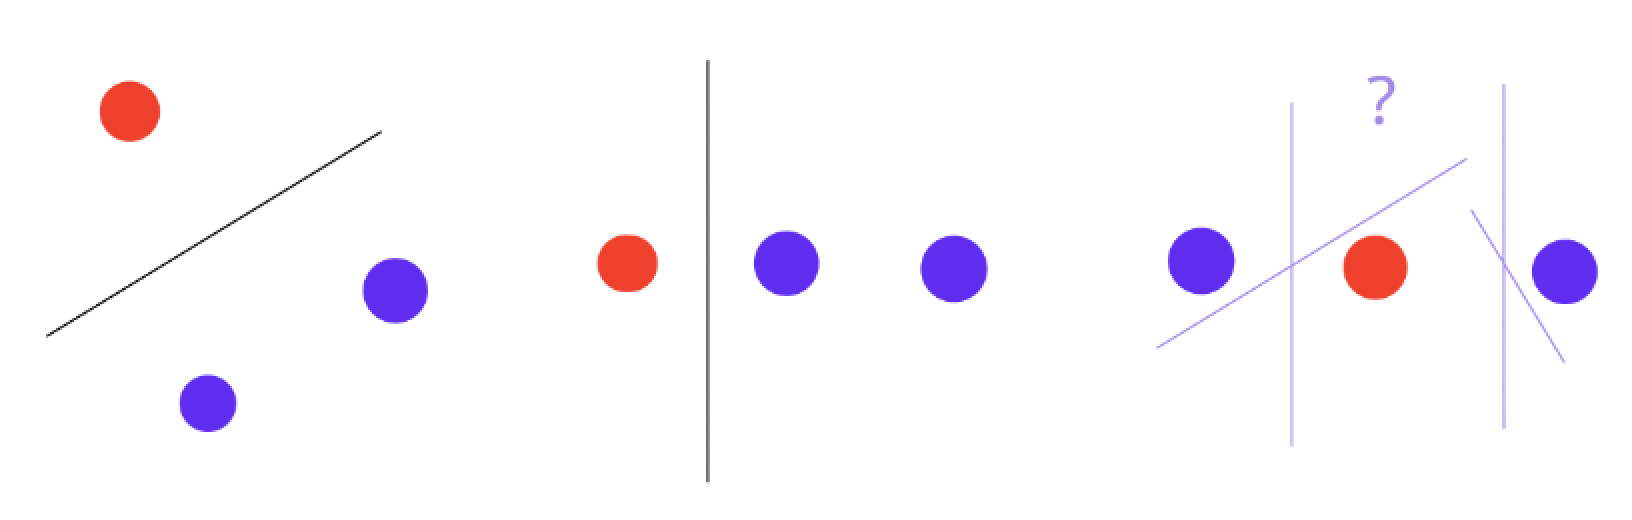
\includegraphics[width=0.6\linewidth]{img/linearly separable.png}
\end{figure}

So, instead of using a linear model, we can use transformed inputs with non-linear relationships with the output, so, for example, we can use a function like the following:

\begin{equation*}
    h_w(x) = w_0 + w_1x + w_2x^2 + \dots + w_mx^m = \sum_{i=0}^m w_ix^i
\end{equation*}

\subsubsection*{Linear Basis Expansion}

This transformation is done by using the \textbf{linear basis expansion (LBE)}:

\begin{equation*}
    h_w(x) = \sum_{k=0}^K w_k\phi_k(x)
\end{equation*}
where each $\phi_k()$ is a function that "transforms" the input; in the previous example, $\phi_0(x)= x^0$, $\phi_1(x)= x^1$, $\phi_2(x)= x^2$, and so on.

Typically, the number of parameters $K$ is greater than $n$.
The model is still linear in the parameters (in $\phi$, not in $x$), so we can still use the same learning algorithm as before, both for regression and classification (by applying the sign function).

\subsubsection{Choosing Phi}
This type of approach is called a "dictionary" approach, since it constructs the linear base expansion out of the function. Using this method can model more complicated relationships (non-linear) since it's more expressive; on the other hand, there's a high risk of overfitting, so we need methods to control the complexity of the model.

\subsubsection{Tikhonov Regularization}
Controlling the complexity can be done in many different ways. One of them is called \textbf{ridge regression (or Tikhonov regularization)}. This method involves adding constraints to the sum of $|w_j|$, penalizing models with high values of $|w|$; i.e., favoring models that use less terms by setting most of the weights to 0 (which results in a simpler model). The loss is calculated as:

\begin{equation*}
    Loss(w) = \sum_{p=1}^l (y_p - x_p^Tw)^2 + \lambda \|w\|^2
\end{equation*}
where $\lambda$ is the regularization hyper-parameter, a small positive value chosen during the model selection phase. Also note that here the name Loss (used for model training) is used to distinguish from Error E (used to evaluate the model error, and corresponding to the data term in this Loss function).

Reformulating the two approaches seen before (direct and iterative), they become as follows:

\begin{itemize}
    \item \textbf{SVD (direct)}: $w = (X^TX + \lambda I)^{-1}X^Ty$

    \item \textbf{Gradient descent (iterative)}: $w_{new} = w + \eta \Delta w - 2\lambda w$ (this is called a weight decay technique; even when the gradient is 0, this addition still reduces the weight by a fraction of it)
\end{itemize}

A balancing can be noted between the value of $\lambda$ and the complexity of the model:

\begin{itemize}
    \item \textbf{Small $\lambda$ value}: the focus is obtaining a small data error term (first term) with a too complex model $\rightarrow $ overfitting;

    \item \textbf{Large $\lambda$ value}: the focus is on the second term, so the data error could grow too much $\rightarrow$ underfitting.
\end{itemize}

The goal is to find the ideal value of $\lambda$ that's neither too small nor too big. We can make a connection between Tikhonov regularization and statistical learning theory; controlling the value of $\lambda$ means controlling the $VC-dim$ of the model, after all: high $\lambda$ means a smaller $VC-dim$ and vice-versa.

\subsubsection{Other Regularization Techniques}

\begin{itemize}
    \item Ridge regression: $\| \|_2$
    \item Lasso: $\| \|_1$
    \item Elastic nets: both $\| \|_1$ and $\| \|_2$
\end{itemize}

The L2 norm penalizes the square value of the weights, and tends to drive all weights to smaller values. L1 norm, on the other hand, penalizes the absolute value of the weights, and tends to drive some weights to exactly 0, but it also introduces a non differentiable loss.

\subsection{Multi-class Task}

\begin{itemize}
    \item \textbf{OVA (one versus all)}: a discriminant function for each class, built on top of real-valued binary classifiers.
    We train $k$ classifiers, each to distinguish the examples in a single class from the examples in any other remaining class; to classify a new example, all $k$ classifiers are run, and the classifier that outputs the largest value is chosen.

    \item \textbf{AVA (all versus all)}: each classifier separates a pair of classes; one classifier for each possible pair. to classify a new example, all the classifiers are run, and the winner is the one with the max sum of outputs or the class with the most votes
\end{itemize}

\section{K-Nearest Neighbor}

The linear model employs an \textbf{eager} learning algorithm: it analyzes the data and constructs an explicit hypothesis capable of generalizing. The final model does not store the training data.

K-Nearest Neighbors instead uses a \textbf{lazy} approach, in which the training data is stored as is; once a new input is presented, it constructs an \textit{ad hoc} hypothesis to classify only that one input.

Its inductive bias is assuming that we can use the distance between points to estimate the output value of a new input.

\subsection{1-Nearest Neighbor}

The simplest possible algorithm. All the training data $TR = <x_p, y_p>$ is stored. Once an input $x$ is received, it finds the nearest neighbor, i.e., the point $x_i$ such that $argmin_i d(x, x_i)$. The distance can be calculated in many different ways (typically euclidean distance). The output for $x$ will be $y_i$, the target value of $x_i$.

This learning algorithm produces a model with no training error, producing decision boundaries that are not linear. Obviously, this leads to overfitting, so the solution is to somewhat increase the training error in order to lessen the generalization error.

\subsection{K-Nearest Neighbors}

Instead of only looking at one neighbor, the output value is calculated by averaging the value of a point's $k$ nearest neighbors. The algorithm first calculates $N_k(x)$, a neighborhood of $x$ that contains $k$ neighbors. Then, the output for regression is calculated as the average target value across that neighborhood:

\begin{equation*}
    h(x) = avg_k(x) = \frac{\sum_{x_i \in N_k(x)} y_i}{k}
\end{equation*}

The output for classification is calculated by majority voting. For a binary classifier it's simply:

\begin{equation*}
    h(x) = \begin{cases}
        1 & avg_k(x) > 0.5 \\
        0 & else
    \end{cases} \, ,
\end{equation*}
or, in the case of multiple classes:
\begin{equation*}
    h(x) = argmax_v \sum_{x_i \in N_k(x)} 1_{v,y_i} \, ,
\end{equation*}
\begin{equation*}
    1_{v,y_i} = \begin{cases}
        1 & v > y_i \\
        0 & else
    \end{cases}
\end{equation*}
The model implicitly uses a \textbf{Voronoi diagram}.

A variant can be used with \textbf{weighted distances}: we may want to add weights to the constribution given by neighbors (i.e. closer neighbors influence the output more than farther ones). So the output for regression is calculated as:

\begin{equation*}
    h(x) = \frac{1}{k}\sum_{x_i \in N_k(x)} \dfrac{y_i}{d(x,x_i)^2} \, ,
\end{equation*}
while the one for classification as:

\begin{equation*}
    h(x) = argmax_v \sum_{x_i \in N_k(x)}  \dfrac{1_{v,y_i}}{d(x,x_i)^2}
\end{equation*}

The main issue in constructing such a model lies in choosing the value of $k$. As seen before, if $k$ is too small, there's overfitting. If $k$ is too big, then both training and generalization errors increase, leading to underfitting.

\subsubsection{Bayes Error Rate}
A Bayes classifier is a learner that uses Bayes' rule to evaluate the most probable output. To find the optimal solution for a classifier, since we know the density $P(x,y)$ (unrealistic situation), we classify to the most probable class: $h(x) = argmax_v P(v|x)$. The error rate of the optimal classifier is called the \textbf{Bayes rate}. It corresponds to the minimum achievable error rate given the distribution of the data.

The K-NN classifier approximates this solution, except that the conditional probability looking at all the data is relaxed to a conditional probability that only refers to a neighborhood of the point, and the actual probability density is unknown.

\subsection{Cons of K-NN}
\begin{enumerate}
    \item \textbf{Scale changes affect the model}: the algorithm does not work as intended is the data is scaled (and thus distances are distorted); the data must be normalized first.

    \item \textbf{High computational cost}: K-NN does not construct a single approximation function; instead, it constructs a new approximation for each input it receives, so the computational cost is completely deferred to the prediction phase. Other than being costly in terms of time (having to calculate distances every time a new input is presented), it's also costly in terms of space, since all the training data must be ready to be used for the prediction.

    \item \textbf{Little space for interpretation}: it's heavily dependent on the metric used.

    \item \textbf{Curse of dimensionality}: as the dimensionality of the data increases, the sparser it becomes, and in turn, the harder it becomes to find the neighbors of a point; and even if found, they would be so far away that the resulting estimate would be no longer local. This would push towards lowering the value of $k$ (so that the estimate depends on closer points), but at the risk of running into overfitting.

    Another relevant issue is that the sampling density ($\frac{l}{volume}$) is proportional to $l^{\frac{1}{n}}$; so, as the dimension grows, the number of points needed to estimate the same function exponentially increases as well.

    Finally, if the target depends only on few of the many features, the output could be influenced by the irrelevant features. This can be solved by either weighting features depending on their relevance, or do feature selection.
\end{enumerate}

\section{Linear Model vs. K-NN Model}

The two models can be considered two extremes:

\begin{table}[h]
    \centering
    \begin{tabular}{c|c}
         Linear & K-NN \\
         \hline
         Rigid & Flexible \\
         Eager & Lazy \\
         Parametric & Instance-based \\
    \end{tabular}
\end{table}

In conclusion, we can say that low variance/ rigidity is poor, but too high variance/ flexibility is dangerous.